\documentclass[border=4pt]{standalone}
\usepackage{lmodern}
\usepackage{amsmath,amssymb}
\usepackage{pgfplots}
\pgfplotsset{compat=1.18}
\begin{document}
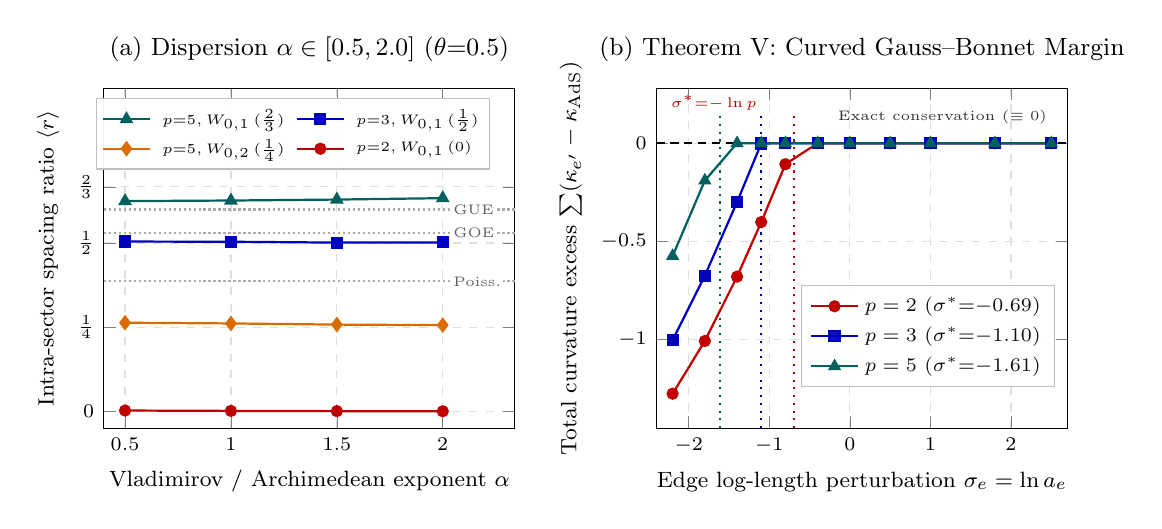
\begin{tikzpicture}
\begin{axis}[
  name=leftplot,
  width=6.8cm,
  height=5.9cm,
  title={\small (a) Dispersion $\alpha \in [0.5, 2.0]$ ($\theta{=}0.5$)},
  xlabel={Vladimirov / Archimedean exponent $\alpha$},
  ylabel={Intra-sector spacing ratio $\langle r \rangle$},
  xmin=0.40, xmax=2.34,
  ymin=-0.05, ymax=0.96,
  xtick={0.5,1.0,1.5,2.0},
  ytick={0,0.25,0.5,0.6667},
  yticklabels={$0$,$\tfrac{1}{4}$,$\tfrac{1}{2}$,$\tfrac{2}{3}$},
  grid=major,
  grid style={dashed, gray!25},
  legend style={at={(0.46,0.97)}, anchor=north, legend columns=2, column sep=2pt, inner sep=2pt, font=\tiny, fill=white, fill opacity=0.95, draw=gray!50},
  legend cell align=left,
  label style={font=\footnotesize},
  tick label style={font=\scriptsize},
]
  \addplot[gray!65, densely dotted, thick, forget plot] coordinates {(0.40, 0.5996) (2.34, 0.5996)};
  \node[anchor=west, font=\tiny, text=gray!75!black, fill=white, inner sep=0.6pt] at (axis cs:2.04, 0.600) {GUE};
  \addplot[gray!65, densely dotted, thick, forget plot] coordinates {(0.40, 0.5307) (2.34, 0.5307)};
  \node[anchor=west, font=\tiny, text=gray!75!black, fill=white, inner sep=0.6pt] at (axis cs:2.04, 0.531) {GOE};
  \addplot[gray!65, densely dotted, thick, forget plot] coordinates {(0.40, 0.3863) (2.34, 0.3863)};
  \node[anchor=west, font=\tiny, text=gray!75!black, fill=white, inner sep=0.6pt] at (axis cs:2.04, 0.386) {Poiss.};

  \addplot[color=teal!75!black, thick, mark=triangle*, mark size=2.1pt] coordinates { (0.5, 0.62455) (1.0, 0.62633) (1.5, 0.62918) (2.0, 0.63336) };
  \addlegendentry{$p{=}5,W_{0,1}\,(\tfrac{2}{3})$}
  \addplot[color=blue!75!black, thick, mark=square*, mark size=1.8pt] coordinates { (0.5, 0.50445) (1.0, 0.50388) (1.5, 0.50134) (2.0, 0.50195) };
  \addlegendentry{$p{=}3,W_{0,1}\,(\tfrac{1}{2})$}
  \addplot[color=orange!85!black, thick, mark=diamond*, mark size=2.2pt] coordinates { (0.5, 0.26334) (1.0, 0.26122) (1.5, 0.25776) (2.0, 0.25623) };
  \addlegendentry{$p{=}5,W_{0,2}\,(\tfrac{1}{4})$}
  \addplot[color=red!75!black, thick, mark=*, mark size=1.8pt] coordinates { (0.5, 0.00255) (1.0, 0.00149) (1.5, 0.00077) (2.0, 0.00035) };
  \addlegendentry{$p{=}2,W_{0,1}\,(0)$}
\end{axis}

\begin{axis}[
  at={(leftplot.east)},
  anchor=west,
  xshift=1.80cm,
  width=6.8cm,
  height=5.9cm,
  title={\small (b) Theorem V: Curved Gauss--Bonnet Margin},
  xlabel={Edge log-length perturbation $\sigma_e = \ln a_e$},
  ylabel={Total curvature excess $\textstyle\sum (\kappa_{e'} - \kappa_{\mathrm{AdS}})$},
  xmin=-2.4, xmax=2.7,
  ymin=-1.45, ymax=0.28,
  xtick={-2,-1,0,1,2},
  grid=major,
  grid style={dashed, gray!25},
  legend style={at={(0.97,0.12)}, anchor=south east, font=\scriptsize, fill=white, fill opacity=0.94, draw=gray!50},
  legend cell align=left,
  label style={font=\footnotesize},
  tick label style={font=\scriptsize},
]
  \addplot[black, densely dashed, thick, forget plot] coordinates {(-2.4, 0) (2.7, 0)};
  % Critical pinch margins sigma* = -ln p
  \draw[red!70!black, dotted, thick] (axis cs:-0.6931, -1.45) -- (axis cs:-0.6931, 0.14);
  \draw[blue!70!black, dotted, thick] (axis cs:-1.0986, -1.45) -- (axis cs:-1.0986, 0.14);
  \draw[teal!70!black, dotted, thick] (axis cs:-1.6094, -1.45) -- (axis cs:-1.6094, 0.14);
  \node[anchor=south, font=\tiny, text=black!80] at (axis cs:1.15, 0.05) {Exact conservation ($\equiv 0$)};
  \node[anchor=south west, font=\tiny, text=red!75!black] at (axis cs:-2.34, 0.12) {$\sigma^* {=} {-}\ln p$};

  \addplot[color=red!75!black, thick, mark=*, mark size=1.8pt] coordinates { (-2.20, -1.27438) (-1.80, -1.00617) (-1.40, -0.67882) (-1.10, -0.40133) (-0.80, -0.10675) (-0.40, 0.00000) (0.00, -0.00000) (0.50, -0.00000) (1.00, -0.00000) (1.80, -0.00000) (2.50, 0.00000) };
  \addlegendentry{$p=2$ ($\sigma^*{=}{-}0.69$)}
  \addplot[color=blue!75!black, thick, mark=square*, mark size=1.8pt] coordinates { (-2.20, -1.00208) (-1.80, -0.67398) (-1.40, -0.29913) (-1.10, -0.00139) (-0.80, -0.00000) (-0.40, -0.00000) (0.00, 0.00000) (0.50, 0.00000) (1.00, 0.00000) (1.80, 0.00000) (2.50, -0.00000) };
  \addlegendentry{$p=3$ ($\sigma^*{=}{-}1.10$)}
  \addplot[color=teal!75!black, thick, mark=triangle*, mark size=2.0pt] coordinates { (-2.20, -0.57398) (-1.80, -0.18999) (-1.40, 0.00000) (-1.10, -0.00000) (-0.80, -0.00000) (-0.40, -0.00000) (0.00, -0.00000) (0.50, -0.00000) (1.00, -0.00000) (1.80, -0.00000) (2.50, -0.00000) };
  \addlegendentry{$p=5$ ($\sigma^*{=}{-}1.61$)}
\end{axis}
\end{tikzpicture}
\end{document}
